\newpage
\section*{Anhang: Messdaten}
\addcontentsline{toc}{section}{Anhang: Messdaten}% Fügt die section dem Inhaltsverzeichnis zu, nummeriert sie aber nicht

\begin{table}
    \centering
    \caption{Abgelesenen Messpunkte zur Auswertung für die Energieverteilung der Elektronen, Teil 1.}
    \label{tab:Energy1}
    \begin{tabular}{S[table-format=1.2] S[table-format=3.1] S[table-format=1.1] S[table-format=1.2] S[table-format=3.1] S[table-format=1.1]}
        \toprule
        $U_\text{A}\,/\,\si{\volt}$ & $I_\text{A}\,/\,\si{\nano\ampere}$ & $\Delta I_\text{A}\,/\,\si{\nano\ampere}$ &
        $U_\text{A}\,/\,\si{\volt}$ & $I_\text{A}\,/\,\si{\nano\ampere}$ & $\Delta I_\text{A}\,/\,\si{\nano\ampere}$ \\
        \midrule
        0.00 & 363.0 & 7.0 & 2.56 & 258.0 & 3.0 \\
        0.08 & 356.0 & 3.5 & 2.64 & 255.0 & 3.0 \\
        0.16 & 352.5 & 3.0 & 2.72 & 252.0 & 3.0 \\
        0.24 & 349.5 & 4.5 & 2.80 & 249.0 & 3.5 \\
        0.32 & 345.0 & 3.0 & 2.88 & 245.5 & 2.5 \\
        0.40 & 342.0 & 4.5 & 2.96 & 243.0 & 3.0 \\
        0.48 & 337.5 & 3.0 & 3.04 & 240.0 & 3.0 \\
        0.56 & 334.5 & 3.0 & 3.12 & 237.0 & 2.5 \\
        0.64 & 331.5 & 3.0 & 3.20 & 234.5 & 3.0 \\
        0.72 & 328.5 & 2.0 & 3.28 & 231.5 & 3.0 \\
        0.80 & 326.5 & 4.5 & 3.36 & 228.5 & 3.0 \\
        0.88 & 322.0 & 2.5 & 3.44 & 225.5 & 2.5 \\
        0.96 & 319.5 & 3.5 & 3.52 & 223.0 & 3.0 \\
        1.04 & 316.0 & 3.0 & 3.60 & 220.0 & 3.0 \\
        1.12 & 313.0 & 3.0 & 3.68 & 217.0 & 3.0 \\
        1.20 & 310.0 & 3.0 & 3.76 & 214.0 & 2.5 \\
        1.28 & 307.0 & 3.5 & 3.84 & 211.5 & 3.0 \\
        1.36 & 303.5 & 3.0 & 3.92 & 208.5 & 3.0 \\
        1.44 & 300.5 & 3.0 & 4.00 & 205.5 & 3.0 \\
        1.52 & 297.5 & 3.0 & 4.08 & 202.5 & 3.0 \\
        1.60 & 294.5 & 3.0 & 4.16 & 199.5 & 3.5 \\
        1.68 & 291.5 & 3.5 & 4.24 & 196.0 & 3.0 \\
        1.76 & 288.0 & 3.0 & 4.32 & 193.0 & 3.0 \\
        1.84 & 285.0 & 3.0 & 4.40 & 190.0 & 3.0 \\
        1.92 & 282.0 & 3.0 & 4.48 & 187.0 & 3.5 \\
        2.00 & 279.0 & 2.5 & 4.56 & 183.5 & 3.0 \\
        2.08 & 276.5 & 3.5 & 4.64 & 180.5 & 3.0 \\
        2.16 & 273.0 & 3.0 & 4.72 & 177.5 & 3.0 \\
        2.24 & 270.0 & 3.0 & 4.80 & 174.5 & 3.5 \\
        2.32 & 267.0 & 3.0 & 4.88 & 171.0 & 3.0 \\
        2.40 & 264.0 & 3.5 & 4.96 & 168.0 & 3.0 \\
        2.48 & 260.5 & 2.5 & 5.04 & 165.0 & 3.5 \\
        \bottomrule
    \end{tabular}
\end{table}
\begin{table}
    \centering
    \caption{Abgelesenen Messpunkte zur Auswertung für die Energieverteilung der Elektronen, Teil 2.}
    \label{tab:Energy2}
    \begin{tabular}{S[table-format=1.2] S[table-format=3.1] S[table-format=1.1] S[table-format=1.2] S[table-format=2.1] S[table-format=1.1]}
        \toprule
        $U_\text{A}\,/\,\si{\volt}$ & $I_\text{A}\,/\,\si{\nano\ampere}$ & $I_\text{A}\,/\,\si{\nano\ampere}$ &
        $U_\text{A}\,/\,\si{\volt}$ & $I_\text{A}\,/\,\si{\nano\ampere}$ & $I_\text{A}\,/\,\si{\nano\ampere}$ \\
        \midrule
        5.12 & 161.5 & 3.5 & 7.12 & 71.0 & 3.0 \\
        5.20 & 158.0 & 3.5 & 7.20 & 68.0 & 4.0 \\
        5.28 & 154.5 & 3.0 & 7.28 & 64.0 & 3.5 \\
        5.36 & 151.5 & 3.5 & 7.36 & 60.5 & 4.5 \\
        5.44 & 148.0 & 3.5 & 7.44 & 56.0 & 3.5 \\
        5.51 & 144.5 & 3.0 & 7.51 & 52.5 & 9.0 \\
        5.59 & 141.5 & 3.5 & 7.59 & 43.5 & 6.0 \\
        5.67 & 138.0 & 3.5 & 7.67 & 37.5 & 7.5 \\
        5.75 & 134.5 & 3.5 & 7.75 & 30.0 & 4.0 \\
        5.83 & 131.0 & 3.0 & 7.83 & 26.0 & 8.0 \\
        5.91 & 128.0 & 3.0 & 7.91 & 18.0 & 7.5 \\
        6.00 & 125.0 & 3.0 & 8.00 & 10.5 & 3.0 \\
        6.08 & 122.0 & 1.0 & 8.08 &  7.5 & 1.5 \\
        6.16 & 121.0 & 4.0 & 8.16 &  6.0 & 1.5 \\
        6.24 & 117.0 & 3.5 & 8.24 &  4.5 & 0.5 \\
        6.32 & 113.5 & 4.0 & 8.32 &  4.0 & 0.5 \\
        6.40 & 109.5 & 7.5 & 8.40 &  3.5 & 0.5 \\
        6.48 & 102.0 & 4.0 & 8.48 &  3.0 & 1.0 \\
        6.55 &  98.0 & 4.5 & 8.56 &  2.0 & 1.0 \\
        6.63 &  93.5 & 4.0 & 8.64 &  1.0 & 1.0 \\
        6.71 &  89.5 & 4.0 & 8.72 &  0.0 & 0.0 \\
        6.79 &  85.5 & 4.5 & 8.80 &  0.0 & 0.0 \\
        6.87 &  81.0 & 4.0 & 8.88 &  0.0 & 0.0 \\
        6.95 &  77.0 & 3.0 & 8.96 &  0.0 & 0.0 \\
        7.04 &  74.0 & 3.0 &      &      &     \\
        \bottomrule
    \end{tabular}
\end{table}
\begin{figure}
    \centering
    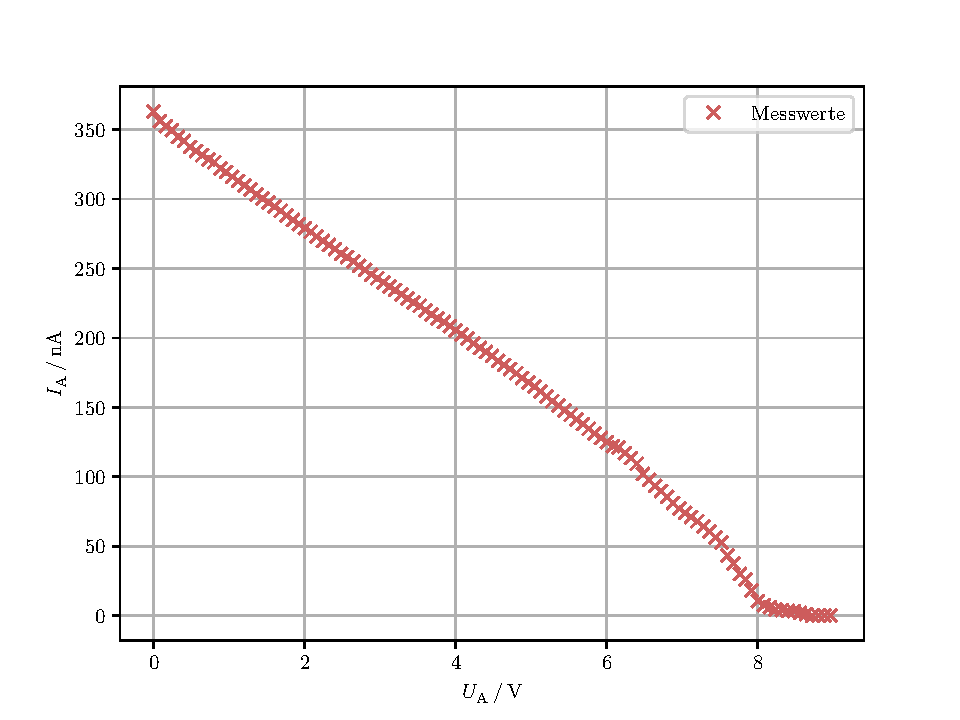
\includegraphics[width=\textwidth]{plots/Energie.pdf}
    \caption{Messwerte zur integralen Energieverteilung der Elektronen.}
    \label{fig:EnergieMess}
\end{figure}
\begin{figure}
    \centering
    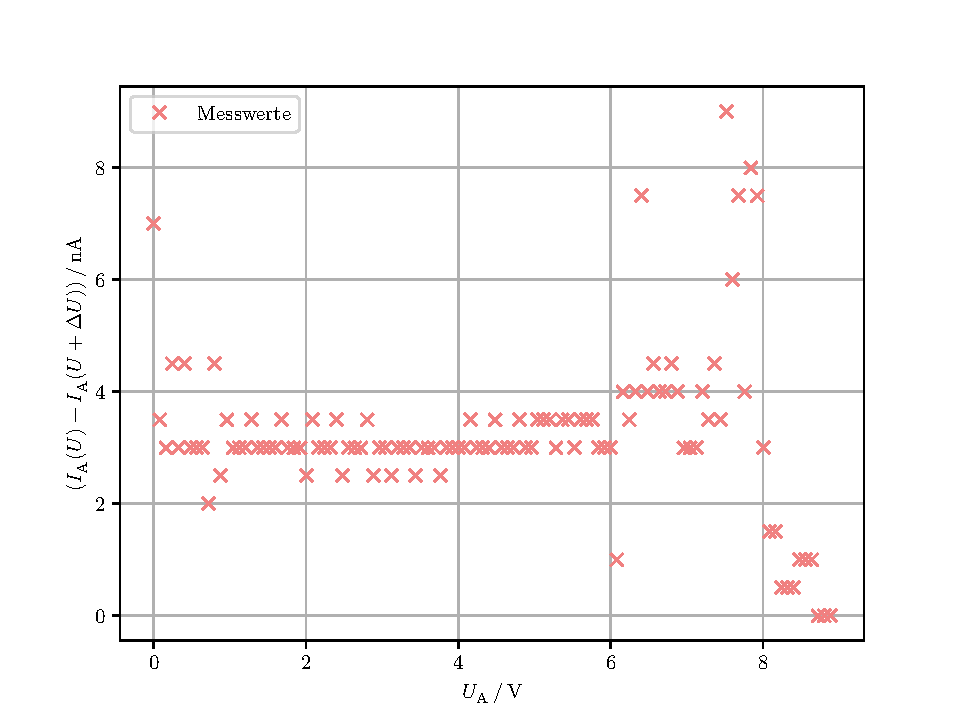
\includegraphics[width=\textwidth]{plots/EnergieDiff.pdf}
    \caption{Messwerte zur differentiellen Energieverteilung der Elektronen.}
    \label{fig:EnergieMess2}
\end{figure}